%-----------------------------------------------------------------------------
%
%               STM paper for SYSTOR'09
%               based on: Template for LaTeX Class/Style File
%
% Template's Author: 
%               Paul C. Anagnostopoulos
%               Windfall Software
%               978 371-2316
%               paul@windfall.com
%
% Used:         31 January 2009
% Created:      15 February 2005
%
%-----------------------------------------------------------------------------


\documentclass[preprint,11pt]{sigplanconf}
% \documentclass[natbib,11pt]{sigplanconf}

\usepackage{amsmath}
\usepackage{graphicx}
\usepackage{listings}
\usepackage[numbers]{natbib}
\usepackage[nohyphen]{underscore}
\usepackage{subfigure}

% code from sigplanconf.cls:
\setlength{\bibsep}{3pt plus .5pt minus .25pt}
%\bibpunct{(}{)}{;}{A}{}{,}
\let \cite = \citep

\begin{document}

\lstset{language=C}
\lstset{basicstyle=\footnotesize\tt, keywordstyle=\tt\bf}

\conferenceinfo{SYSTOR '09}{4-6 May 2009, Haifa, Israel.} 
\copyrightyear{2009} 
\copyrightdata{[to be supplied]} 

\titlebanner{DRAFT - Do not distribute}        % These are ignored unless
\preprintfooter{Transactifying Apache}         % 'preprint' option specified.

\title{Transactifying Apache}
% \subtitle{Subtitle Text, if any}

\authorinfo{Haggai Eran\and Ohad Lutzky\and Zvika Guz\and Idit Keidar}
           {Department of Electrical Engineering, Technion - Israel Institute of Technology}
           {haggaie@tx.technion.ac.il\and lutzky@gmail.com\and zguz@tx.technion.ac.il\and idish@ee.technion.ac.il}
%\authorinfo{Name2\and Name3}
%           {Affiliation2/3}
%           {Email2/3}

\maketitle

\begin{abstract}
Apache is a large-scale industrial multi-process and multi-threaded
application, which uses lock-based synchronization. We report on our
experience in modifying Apache to employ transactional memory instead of
locks, a process we refer to as \emph{transactification}; we are not
aware of any previous efforts to transactify legacy software of such
a large scale. Along the way, we learned some valuable lessons about
which tools one should use, which parts of the code one should
transactify and which are better left untouched, as well as on the
intricacy of commit handlers. We also stumbled across weaknesses of
existing software transactional memory (STM) toolkits, leading us
to identify desirable features they are currently lacking.
Finally, we present performance results from running
Apache on a 32-core machine, showing that, there are scenarios
where the performance of the STM-based version is close to that of the
lock-based version.  These results suggest that there are applications for which
the overhead of using a software-only implementation of transactional memory is
insignificant.
\end{abstract}

\category{D.1.3}{Programming Techniques}{Concurrent Programming}

\terms
Measurement, Performance, Experimentation

\keywords
Software Transactional Memory

\section{Introduction}

The vast shift to multi-core machines in recent years 
creates a major challenge for software developers, 
who must learn how to exploit the parallelism that such
architectures can offer.
In this context, \emph{Transactional Memory (TM)} is one of the leading
paradigms targeted at allowing programmers to easily harness the 
parallelism of future multi-core machines and to extract the 
performance promise these systems can offer. 
Since hardware transactional memory implementations are not
yet in the market,  \emph{Software Transactional Memory (STM)} tools
offer a viable alternative in the interim. 

One of the principal challenges that TM systems confront, (besides 
delivering performance), is the ability to handle large-scale commercial applications.
Developers that wish to employ TM, face the challenge of 
applying it to large legacy code. As TM systems are maturing, these aspects of 
convertibility and completeness are becoming critical in order to allow TM to shift from 
a promising concept to a full-fledged commercial tool. In this work, we try, via a design 
example, to answer how far we are from achieving these goals. 

To date, TM was mostly employed within the niche of complex
concurrent data structures, such as red-black trees and skip lists
\cite{herlihy:DSTM, fraser:practical:thesis:2003}, and isolated scientific
algorithms (such as STAMP~\cite{caominh:stamp:iiswc:2008});
it was additionally used for  benchmarks such as
STMBench7~\cite{STMBench7}, which measures operations on a complex yet still
artificial object graph.
Moreover, Transactional Memory was mostly used thus far in benchmarks that 
were implemented explicitly with TM from the outset. 

In this paper, we use Transactional Memory
for the first time in the context of large-scale industrial software, which,
moreover, does not pertain to any of the typical niches of transactional memory
benchmarks. Furthermore, we convert legacy code, which used lock-based
synchronization, to work with transactional memory, rather than write the
benchmark from scratch. We refer to this conversion process as
\emph{transactification}. Specifically, we transactify the Apache 
web server. Since Apache is written in C, we needed to employ C-based
STM toolkits. We next recognized that it would not be feasible to
use \emph{library-based} STM tools, as this  
would entail changing all reads and writes to global variables in the code.
Instead, we opted for \emph{compiler-based} STMs. 
We experimented with two such tools, 
{\sc Tanger}~\cite{felber2007tanger} and Intel's STM Compiler~\cite{icc}.
Section~\ref{sec:background} provides background on Apache
and the two STM tools we attempted to use in this endeavor. 

Our goal in this exercise is twofold. First, we wanted to examine whether the transactional 
memory paradigm is broadly applicable, outside its traditional niches, in contexts where a 
high level of parallelism is already obtained using lock-based synchronization. 
%[XX Can we 
%quote something somebody said before on where it should not work?? XX]. 
%
Second, as transactional memory is being touted as the panacea for the limited parallelism 
of coarse-grained locks, and since coarse-grained locks that limit parallelism are widely used 
in legacy code, one can anticipate a growing need for transactification of legacy software. 
We sought to learn how painful such a process can be, and what can be done in order to 
facilitate it.

In the course of this project, we learned some valuable lessons.
For example, we have seen that tools vary in the features they are able
to support, which has significant impact on their usability in 
such large-scale projects. We have further learned that in such a large
system, it is more realistic to transactify only pertinent parts of the code,
while most of the code is better left untouched. Finally, we have found
that there is a vital need to sometimes defer irrevocable actions to
the end of a transaction; this feature is provided by a language construct called 
a \emph{commit handlers}. In Section~\ref{sec:transactification}, 
we describe in detail our transactification
process, including the hurdles we have encountered and the means used to
overcome them.

Though we finally managed to overcome the hurdles and create working transactified 
code, the process left us somewhat unsatisfied with the current state of the art. 
In Section~\ref{sec:wishlist}, we compile a \emph{wish list} of features 
that would have been very helpful in this process, had they been provided
by TM toolkits; we hope that developers of future STM versions
will take these into consideration. 

In Section~\ref{sec:evaluation} we study the performance of the transactified 
version of Apache on a 32-core machine. 
Note that since the legacy Apache code is already 
tuned to work well with multiple threads and multiple processes, 
and since we use software-only TM solutions, which were not optimized for this 
application, one could expect the transactified version to be significantly
slower than the original.
Somewhat surprisingly, we show that this is not the case, and the 
transactified 
version's performance is competitive to that of the lock-based legacy code. 
As future TMs are expected to incorporate hardware support, and also 
to be better optimized for a range of application, our results 
suggests that in the future, porting applications to TM may be valuable.

Section~\ref{sec:conclusions} summarizes the lesson we learned in the 
transactification process.

\section{Background: Software and Tools}
\label{sec:background}

\subsection{Apache}\label{sec:apache}

Apache~\cite{apache} HTTP server is a popular web server application written in
C. It supports working on multiprocessor machines with several multi-processing
modules (MPMs) each offering a different strategy for handling requests and
distributing the work. The most popular threaded MPM is the \emph{worker} MPM,
which works by running multiple worker-threads under several processes, each
thread handles a single request at a time. In each such process there are
several worker threads, and also a listener thread that fetches incoming
requests and dispatches them to the available workers, as illustrated in
Figure~\ref{fig:apache-worker-MPM}.

\begin{figure}
 \begin{center}
  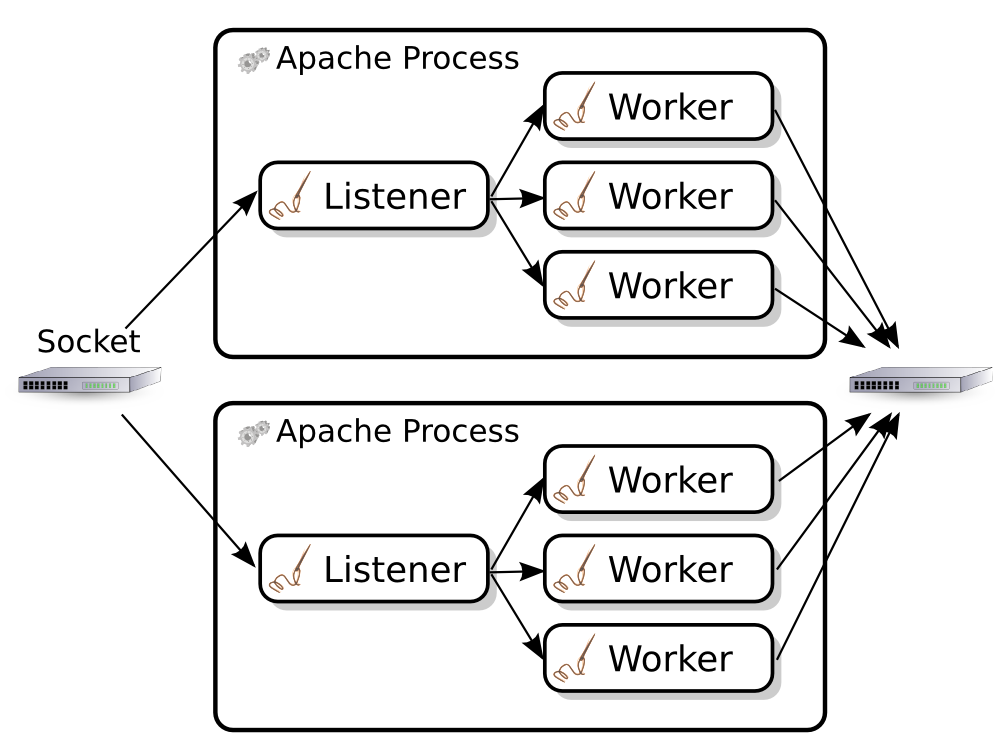
\includegraphics[width=8cm]{Apache-Worker-MPM.png}
 \end{center}
 \caption{Apache worker MPM architecture.}
 \label{fig:apache-worker-MPM}
\end{figure}

There are not many points of interaction between the worker threads themselves,
where transactional memory can be used. One such place is Apache's memory cache
implemented by the {\tt mod\_mem\_cache} module. This module enables the workers
of each process to share a cache of recently served requests. A new request can
be served from the memory cache, and save the time required to access the disk
and generate the requested page. Since the cache is shared among multiple
threads, it is synchronized by a single lock, therefore a good candidate for
converting into transactional memory.

Apache's cache is implemented with a couple of modules. The first, {\tt
mod\_cache}, implements the logic related to caching. It tests the metadata of
each requests to see if it can be supplied from the cache, according to the
request's HTTP headers and the system configuration. It uses one of the
underlying cache implementation modules, {\tt mod\_mem\_cache} or {\tt
mod\_disk\_cache} to do the actual caching.

The {\tt mod\_mem\_cache} module implements a memory cache using a shared hash
table and priority queue. The key to the hash table is the URL of the request,
converted into a canonical form. The cache is limited both by size and by the
number of elements, and by memory size, so on insertion, sometimes lower
priority entries are removed from the cache. The priority is determined by one
of two algorithms: LRU, removing the least recently used entries first, and GDSF
(Greedy Dual Size Frequency) assigning score to entries based on the cost of a
cache miss, and the entry size.

\subsection{C STM Systems}

C and C++ STM systems divide into two kinds: Library based and compiler based.
Library based STMs \cite{TL2,felber2008tinystm,RSTM} are built as a C library.
Every transaction begins with a call into the library, and commits by another
call. All reads and writes to global variables must be done through special
library functions when in a transaction. This requires a great amount of work
for converting an application to use STM. Not only accesses to global memory in
the function that started the transaction must be converted, but also any access
from any function being called from this function. We therefore ruled out
this approach. 

In contrast, compiler-based STM
\cite{felber2007tanger,icc,gcctm,baek:opentm:pact:2007} use a specialized
compiler, which has extended syntax for transactional memory atomic blocks. The
compiler can then automatically convert memory accesses inside transactions
into calls to the underlying library. The term \emph{transactification}
sometimes refer to this process. We experimented with two compiler-based
STMs, which we now describe. 

\subsubsection{Tanger}
The {\sc Tanger}~\cite{felber2007tanger} transactifying compiler is an
open-source academic compiler extension for LLVM~\cite{LLVM:CGO04}, an
extensible compiler framework.  Tanger aims at creating a transactifying
compiler that is independent of the STM system used. It works with the
TinySTM~\cite{felber2008tinystm} library, but can easily be extended to use
other STM libraries by writing a simple plugin.

{\sc Tanger} is accompanied with the {\sc Tarifa}~\cite{felber2007tanger}
tool, which transactifies compiled binaries, even without the sources. This
feature is a very important advantage when modifying legacy code, where often
not all the source code is available, as the code uses legacy libraries.

\subsubsection{Intel STM Compiler}

Intel has published~\cite{icc} an experimental STM compiler based on their industrial
compiler ICC. Although ICC uses a proprietary STM manager, Intel has published their
ABI~\cite{icc:abi} allowing for other STM managers to replace their own. This feature
and its selective transactification ability were the main reasons why we
preferred ICC.

In the latest version of Intel STM Compiler, support for abort and commit
handlers was also added to the system, by registering a callback function
from inside a transaction.

An extension to the Gnu Compiler Collection (GCC) is being developed~\cite{gcctm} to
enable transactional memory support for GCC. It is intended to work with
TinySTM, but being open source, other STM systems will probably be ported too.
The syntax of the C/C++ language extensions is designed to be compatible with
ICC. This means that applications converted for ICC will probably be compilable
under GCC with this extension, without much modification.

\section{Transactification}\label{sec:transactification}
\subsection{Which STM to use?}

On examining the Apache code, our first observation was that
the vast majority of the code does not access any global variables,
and therefore does not require transactification at all.
Upon identifying the parts that do require atomicity,
we wanted to only focus on them, without touching
the rest of the code, in order to save work for the programmers
as well as saving unnecessary work for the compiler and the linker.

We first attempted to do this with {\sc Tanger}, albeit unsuccessfully.
The version of {\sc Tanger} we used
created a transactified version of each function in a compilation
unit.  Every function call inside a transaction was then converted to a call to
the new version. This creates a major disadvantage when working on a large
application. Moreover, sometimes the
transactification might fail because of calls to functions whose source is not
available and cannot be transactified. This can cause the entire build process
to fail, where in fact the code could have been transactified without any error
by skipping these functions.

This drawback was the main reason why we eventually chose to use Intel's STM
Compiler. It solves the unneeded transactification problem by adding some new function attributes
to the language in order to tell the compiler which functions need to be transactified.
The attribute {\tt tm\_callable} tells the compiler that a transactified version
of the function will be needed. This way, only functions that are required inside
transactions can be marked as {\tt tm\_callable} and be transactified.

Lately, a new release of {\sc Tanger} was announced, one in which the developer
can annotate which functions should be transactified. However, we did not get a
chance to try it.

\subsection{What to transactify}
We have decided to focus our change in Apache with the memory cache module. As
described in Section \ref{sec:apache}, it is a significant point of interaction
between Apache's worker threads, and since it is implemented with a course-grained
lock, it is ideal for converting into STM. Another advantage is that it is a
well encapsulated module, allowing us to study the effect of converting a small 
part of code on the larger system -- Apache itself has about 340,000 lines of
code, while the cache module is comprised of only 6651 lines of code.

The conversion process included converting critical sections protected by the
cache module's main lock into atomic blocks, and decorating required functions
as {\tt tm\_callable}. The module had used atomic instructions for some memory
accesses, and these were converted to full transactions in atomic blocks, so
that collisions with these accesses will be detected. Overall we only changed
273 lines of code, some in the cache module, and some with additional helper
functions such as the atomic instruction wrappers.

\subsection{Defining atomic blocks}
\begin{figure*}
\lstset{emph={apr_thread_mutex_lock, apr_thread_mutex_unlock, apr_pool_cleanup_register}, emphstyle=\bf}
\begin{lstlisting}
static int open_entity(cache_handle_t *h, request_rec *r, const char *key) {
  ...
  if (sconf->lock) apr_thread_mutex_lock(sconf->lock);

  obj = (cache_object_t *) cache_find(sconf->cache_cache, key);
  if (obj) {
    if (obj->complete) {
      request_rec *rmain=r, *rtmp;
      apr_atomic_inc32(&obj->refcount);
      /* cache is worried about overall counts, not 'open' ones */
      cache_update(sconf->cache_cache, obj);

      /* If this is a subrequest, register the cleanup against the main
       * request.  This will prevent the cache object from being cleaned up
       * from under the request after the subrequest is destroyed. */
      rtmp = r;
      while (rtmp) {
        rmain = rtmp;
        rtmp = rmain->main;
      }
      apr_pool_cleanup_register(rmain->pool, obj, decrement_refcount, 
        apr_pool_cleanup_null);
    }
    else obj = NULL;
  }

  if (sconf->lock) apr_thread_mutex_unlock(sconf->lock);
  ...
}
\end{lstlisting}
\caption{Original {\tt open\_entity} function.}
\label{code:original-open-entity}
\end{figure*}

Following the conversion, some transactions contained code that pertained to
the transaction, but did not necessarily need to run atomically with the
transaction. An example might be a transaction removing an object from the
cache, and freeing its memory. While the removal operation must be protected
inside a transaction as it is using the shared memory structure of the cache,
the memory release can happen any time later, since no other thread can point to
the removed object after it had been removed from the cache. 

For lock based systems, having the memory release as part of the critical
section might cause a thread to hold the critical section a little longer than
needed, but does not cause any problems other than that. In TM
systems, including the memory release in the transaction slows down
the system in a similar way, since
having accesses to memory structures such as those required by
memory management may cause collisions with other threads. But 
in addition, with this approach, the cleanup functions need to be
transactified, which requires additional work both from the programmer and the
compiler.

In our case, we chose not to transactify such functions, but instead remove them
from the atomic section, and execute them after the transaction had committed.
Although this requires some changes to the code, the changes are limited to the
call-site, and need not modify any of the called libraries.

For example, the  critical section in the {\tt open\_entity} function
shown in Figure~\ref{code:original-open-entity}
 is responsible for retrieving a page
to fulfill a request from the server. It  increments the reference count on
the cached page, and registers a decrement function to be invoked upon completing
the request. When we converted the critical section into a transaction, we
did not want the function {\tt apr\_pool\_cleanup\_register} to be called from
inside the transaction, as transactifying it would require working on another
library, the Apache Portable Runtime library, thus breaking encapsulation.

The semantics of requests and sub-requests in Apache guarantee the request
cannot be completed before the return of this function, therefore we could
move the registration of the cleanup function out of the atomic section, as 
seen in Figure~\ref{code:transactified-open-entity}. In this example, 
the registration occurred at the end of the atomic block, so 
we did not have to move it in order to take it out of the block;
we simply ended the atomic block earlier. Nevertheless, in other cases,
such actions occur in the middle of an atomic block. For example, in a function
that cleans up multiple objects from the cache, for of the objects removed it
would first remove its pointer from the cache, and then decrease its reference
count in free its memory if necessary. In this case we would like to do all the
removals inside the transaction, and all the reference decrements and memory
cleanup oustide of the transaction. In order to deal with such scenarios, it is
desirable to have language support for commit handlers, as explained in the next
section. 

\begin{figure*}
\lstset{emph={__tm_atomic, apr_pool_cleanup_register}, emphstyle=\bf}
\begin{lstlisting}
static int open_entity(cache_handle_t *h, request_rec *r, const char *key)
{
  ...
  __tm_atomic {
    obj = (cache_object_t *) cache_find(sconf->cache_cache, key);
    if (obj) {
      if (obj->complete) {
        ++obj->refcount;
        /* cache is worried about overall counts, not 'open' ones */
        cache_update(sconf->cache_cache, obj);
      }
      else obj = NULL;
    }
  }

  /* Register the object for updating after cleanup */
  if (obj && obj->complete) {
    request_rec *rmain=r, *rtmp;
    /* If this is a subrequest, register the cleanup against the main
     * request.  This will prevent the cache object from being cleaned up
     * from under the request after the subrequest is destroyed.  */
    rtmp = r;
    while (rtmp) {
      rmain = rtmp;
      rtmp = rmain->main;
    }
    apr_pool_cleanup_register(rmain->pool, obj, decrement_refcount, 
      apr_pool_cleanup_null);
  }
  ...
}
\end{lstlisting}
\caption{Transactified {\tt open\_entity} function.}
\label{code:transactified-open-entity}
\end{figure*}

\subsection{Commit Handlers}
Commit and undo handlers are pieces of code that are scheduled by a transaction
to run when the transaction will commit, or abort, respectively. This mechanism,
was suggested in~\cite{tm:commit-handlers}.  Commit handlers are described
there as a mechanism that allows finalization of tasks, for instance, a
transactional system call such as write to file might have its permanent side
effects be executed in a commit handler. 
Abort handlers are called when a transaction is aborted and can reverse the 
side-effects of a transaction. 

These handlers can sometimes be used to implement
more efficient transactions. For example, if allocating memory inside a
transaction, (assuming without a specialized memory allocator which is available
in many STMs), the STM would need to log all the memory accesses to the memory
management data structures, and undo these writes in case of an abort. A more
efficient solution could be allocating the memory immediately, and in case of an
abort just free the memory in an abort handler.

 From our perspective, commit handlers could have been used to make the
modifications we wanted in the atomic blocks, and move finalization functions
out of atomic blocks just by registering them as commit handlers. In the 
example shown in Figure~\ref{code:original-open-entity}, 
the call to {\tt apr\_pool\_cleanup\_register} could have been
converted into a call registering this function as a commit handler. 

Intel STM Compiler support abort and commit handlers in its latest addition.
Handlers are written as functions with a single {\tt void~*} argument, and
registered by calling the API functions {\tt \_ITM\_add\-User\-Commit\-Action} or
{\tt \_ITM\_add\-User\-Undo\-Action}. This feature was only recently added, and we have
not used it in our experiments. {\sc Tanger} currently does not support
registering such handlers.

\section{Wish List}\label{sec:wishlist} 

During the transactification process, we have identified several apparatus whose
absence has complicated the conversion process. In this section, we indicate
several such issues in the hope that this will expedite their assimilation into
future STMs.

\subsection{Handler Closures}
\begin{figure*}
\lstset{emph={__tm_atomic, apr_pool_cleanup_register, on_commit}, emphstyle=\bf}
\begin{lstlisting}
static int open_entity(cache_handle_t *h, request_rec *r, const char *key) {
  ...
  __tm_atomic {
    obj = (cache_object_t *) cache_find(sconf->cache_cache, key);
    if (obj) {
      if (obj->complete) {
        request_rec *rmain=r, *rtmp;
        ++obj->refcount;
        /* cache is worried about overall counts, not 'open' ones */
        cache_update(sconf->cache_cache, obj);

        /* If this is a subrequest, register the cleanup against the main
         * request.  This will prevent the cache object from being cleaned
         * up from under the request after the subrequest is destroyed. */
        rtmp = r;
        while (rtmp) {
          rmain = rtmp;
          rtmp = rmain->main;
        }
        on_commit {
          apr_pool_cleanup_register(rmain->pool, obj, decrement_refcount, 
            apr_pool_cleanup_null);
        }
      }
      else obj = NULL;
    }
  }
  ...
}
\end{lstlisting}
\caption{{\tt open\_entity} function with desired commit handler closure syntax.}
\label{code:closure-open-entity}
\end{figure*}

While commit handlers can aid a lot in the process of transactifying a legacy
application, their current syntax in Intel STM Compiler is very limiting.
Handlers must be given as a pointer to function of a specific signature, so a
developer trying to move a piece of code out of an atomic block, would still
need to write a new function. It would be nice to have a language construct that
defines a new commit handler right where it is being registered, however this
requires the language to support closures. 

A closure is a function that has bounded variables from the environment where it
was defined. It is intended to be passed along similarly to a function pointer,
and when called refer to variables that existed where it was defined. In
Figure~\ref{code:closure-open-entity}, we give an example of the desired syntax
of such a commit handler closure. The block of code after the {\tt on_commit}
keyword uses variables such as {\tt rmain} and {\tt obj} from its surrounding
block that must be captured until it is executed later when the transaction
commits.

Having closures allows us to easily defer execution of code until after the
transaction commits, with minimal modification to our code. Instead of creating
a new function for each piece of code being deferred, and possible create new
data types to hold the data from inside the transaction that each such function
required, with closures we could just change the piece of code being deferred
into a closure, and let the implementation handle these tasks.

Of course there are many problems implementing closures in a language without
garbage collection such as C, especially since there is no guarentee that the
pointers taken by the closure will not be invalidated before the closure is run.

% \clearpage

\subsection{Statistics and Profiling}\label{sec:wishlist-statistics}
Intel's STM manager collects statistics about the transactions being run, their
size, abort rates, etc. Unfortunately however, it cannot work with a
multiprocess application such as Apache. This limits the ability to investigate
the performance of converted applications to only limited runs with only one
process, or having only black box measurements of the system.

Collecting these statistics ourselves was not possible without abort handlers,
of course, because any statistics data a transaction might modify would be
reset to its original value in case the transaction aborted. Abort handlers
allow us to track these measurements ourselves, but since they were only
added in Intel's latest compiler, we have not implemented such measurements yet.

\section{Performance Evaluation}\label{sec:evaluation}
\subsection{Methodology} 

We evaluate the transactified web server  using \emph{Siege} \cite{siege}, an
HTTP load testing tool. The server is loaded with the set of UNIX man-pages -- a
set of small textual files typical of some web sites. Each page is served using
the \emph{man2html} program, uncompressed and converted into HTML.
Thus,  
the serving of files requires enough computational resources to make the use of
caching worthwhile.

The man2html program is a Common Gateway Interface (CGI) program that serves
unix manual (man) pages on Internet sites. The pages are usually stored
compressed in gzip format, and formatted using the troff format. The program
receives a request for a man page from the web server, uncompresses the required
file, and converts it to HTML. As every CGI program, it outputs the result with
relevant HTTP headers.

The default caching policy of Apache forbids caching dynamically generated pages
such as those of man2html, unless the HTTP headers of the resulting page clearly
specify otherwise. To make caching of the man2html pages possible, we modified
man2html to output such headers, specifying the output can be cached for one
hour.

In each experiment, the pages are requested randomly according to a Zipf 
distribution with some parameter $s$, which
determines how frequently the most popular pages are visited,
thus controlling the level of locality in the requests.
The higher the value of $s$ is, the more locality there is in the 
workload.

The experiments run on two computers connected by  Gigabit Ethernet.
Each of the machines is an 8-processors SMP, with quad core 2.3GHz AMD Opteron
processors (for a total of 32 cores), and 126GB of RAM. One of the machines was
used as a server running Apache, and the other served as a client, running
Siege.

\subsection{Results} 

\begin{figure*}
 \centering
 \subfigure[Request throughput]{
  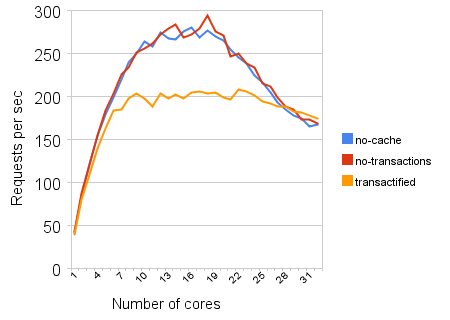
\includegraphics[width=8.5cm, trim=1cm 9.5cm 0 10.6cm]{transaction-rate-client-server-0dot1.pdf}
  \label{fig:request-throughput-0.1}
 }
 \hfill
 \subfigure[Average response time]{
  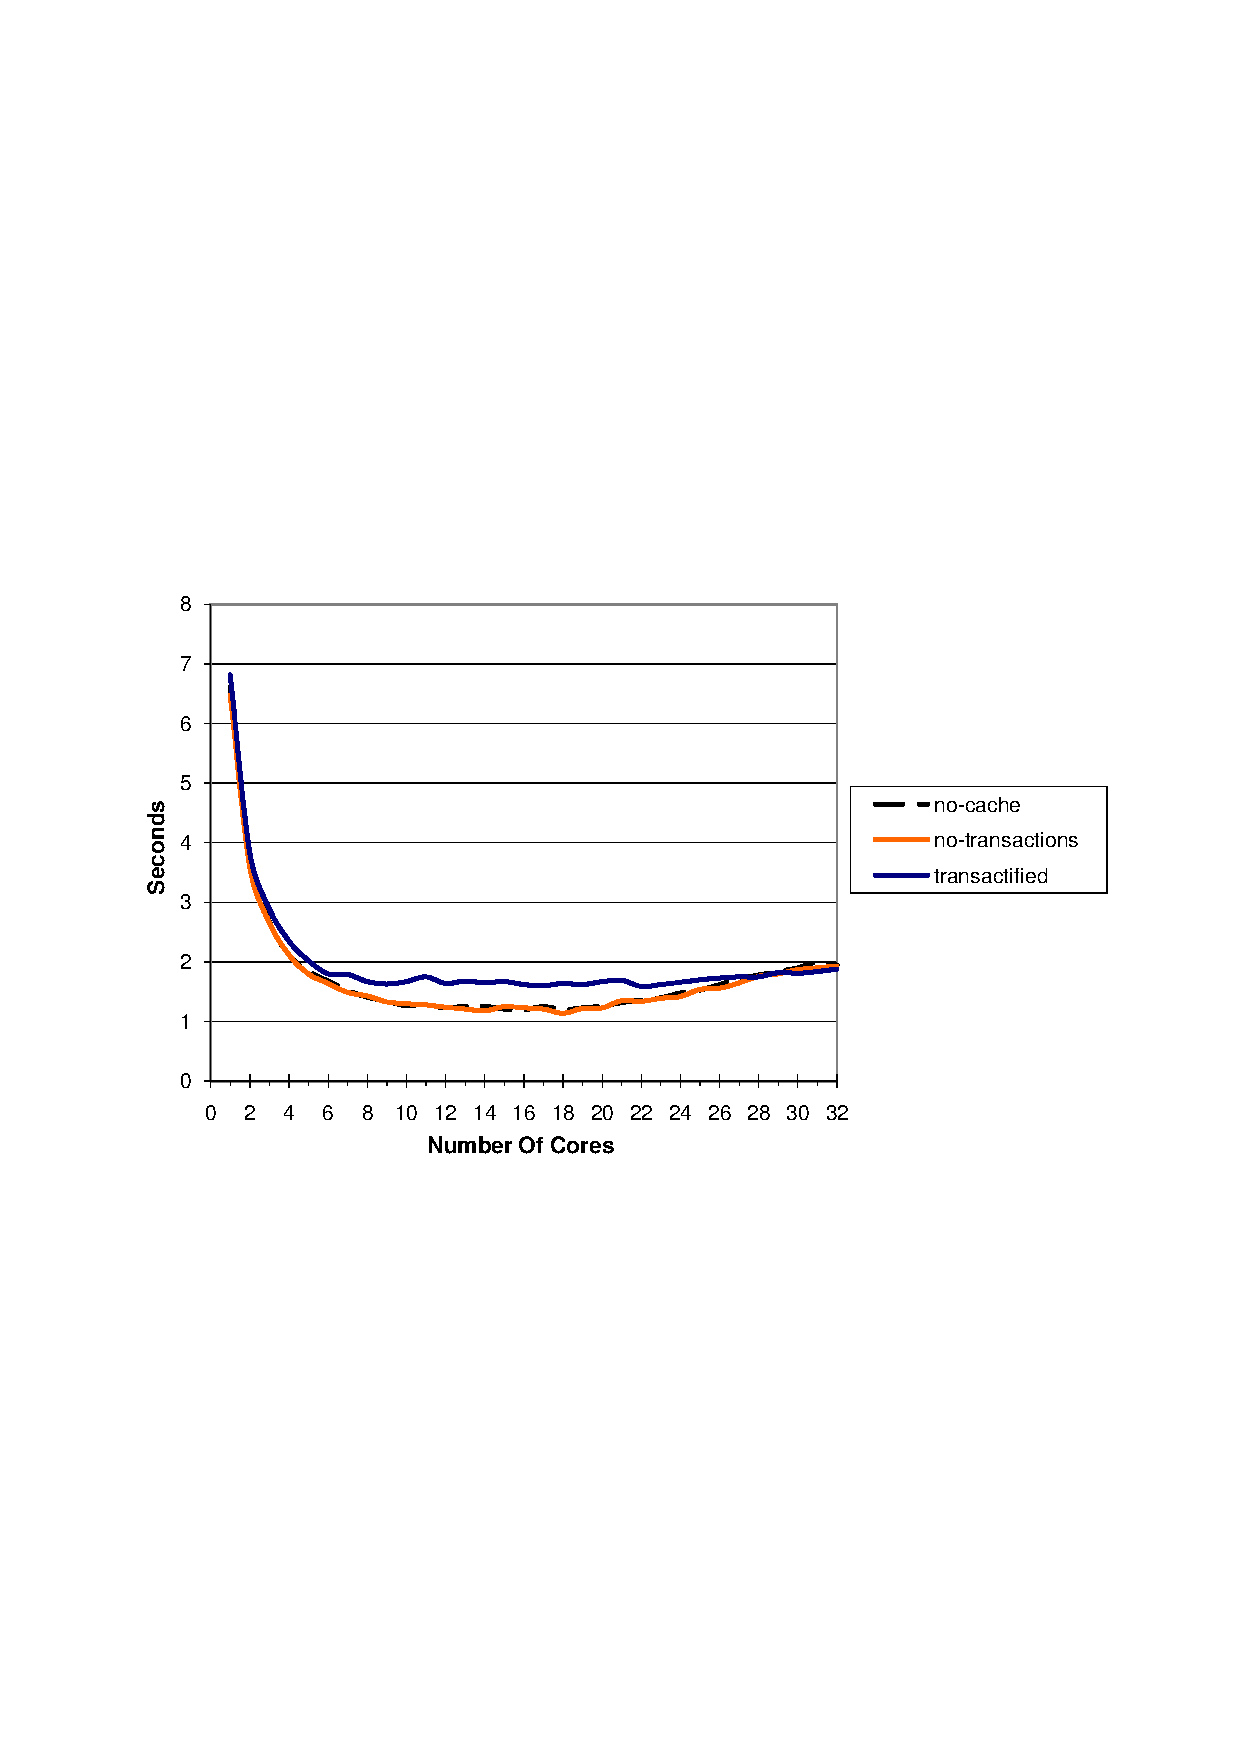
\includegraphics[width=8.5cm, trim=1cm 9.5cm 0 10.6cm]{response-time-client-server-0dot1.pdf}
  \label{fig:response-time-0.1}
 }
 \caption{Very low locality workload ($s = 0.1$). The cache is not effective,
 and the penalty of using STM is high.}
\end{figure*}

We compare the average latency and request throughput when running on different
numbers of cores, and with different  values of $s$. Each graph presents 
results from three
experiments, comparing the performance of an Apache server running without a cache, a
cached version without our transactional modifications, and the transactified
version. 

As expected, with low locality ($s=0.1$), the cache yields almost no benefit.
Moreover, the penalty of
the STM increases with the number of processors, causing it to be less
practical, as we see in Figures~\ref{fig:request-throughput-0.1}
and~\ref{fig:response-time-0.1}. This degradation of the STM-based version
occurs since almost all of the requests result in cache
misses, thus causing more work to be done within transactions, 
and increasing contention.  However, this workload is not representative;
typical Apache workloads exhibit more locality, and hence benefit from
the cache.

\begin{figure*}
 \centering
 \subfigure[Request throughput]{
  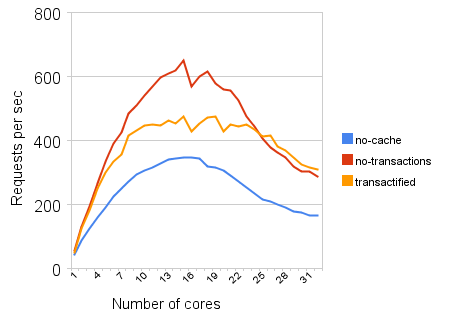
\includegraphics[width=8.5cm, trim=1cm 9.5cm 0 10.6cm]{transaction-rate-client-server-1.pdf}
  \label{fig:request-throughput-1}
 }
 \hfill
 \subfigure[Average response time]{
  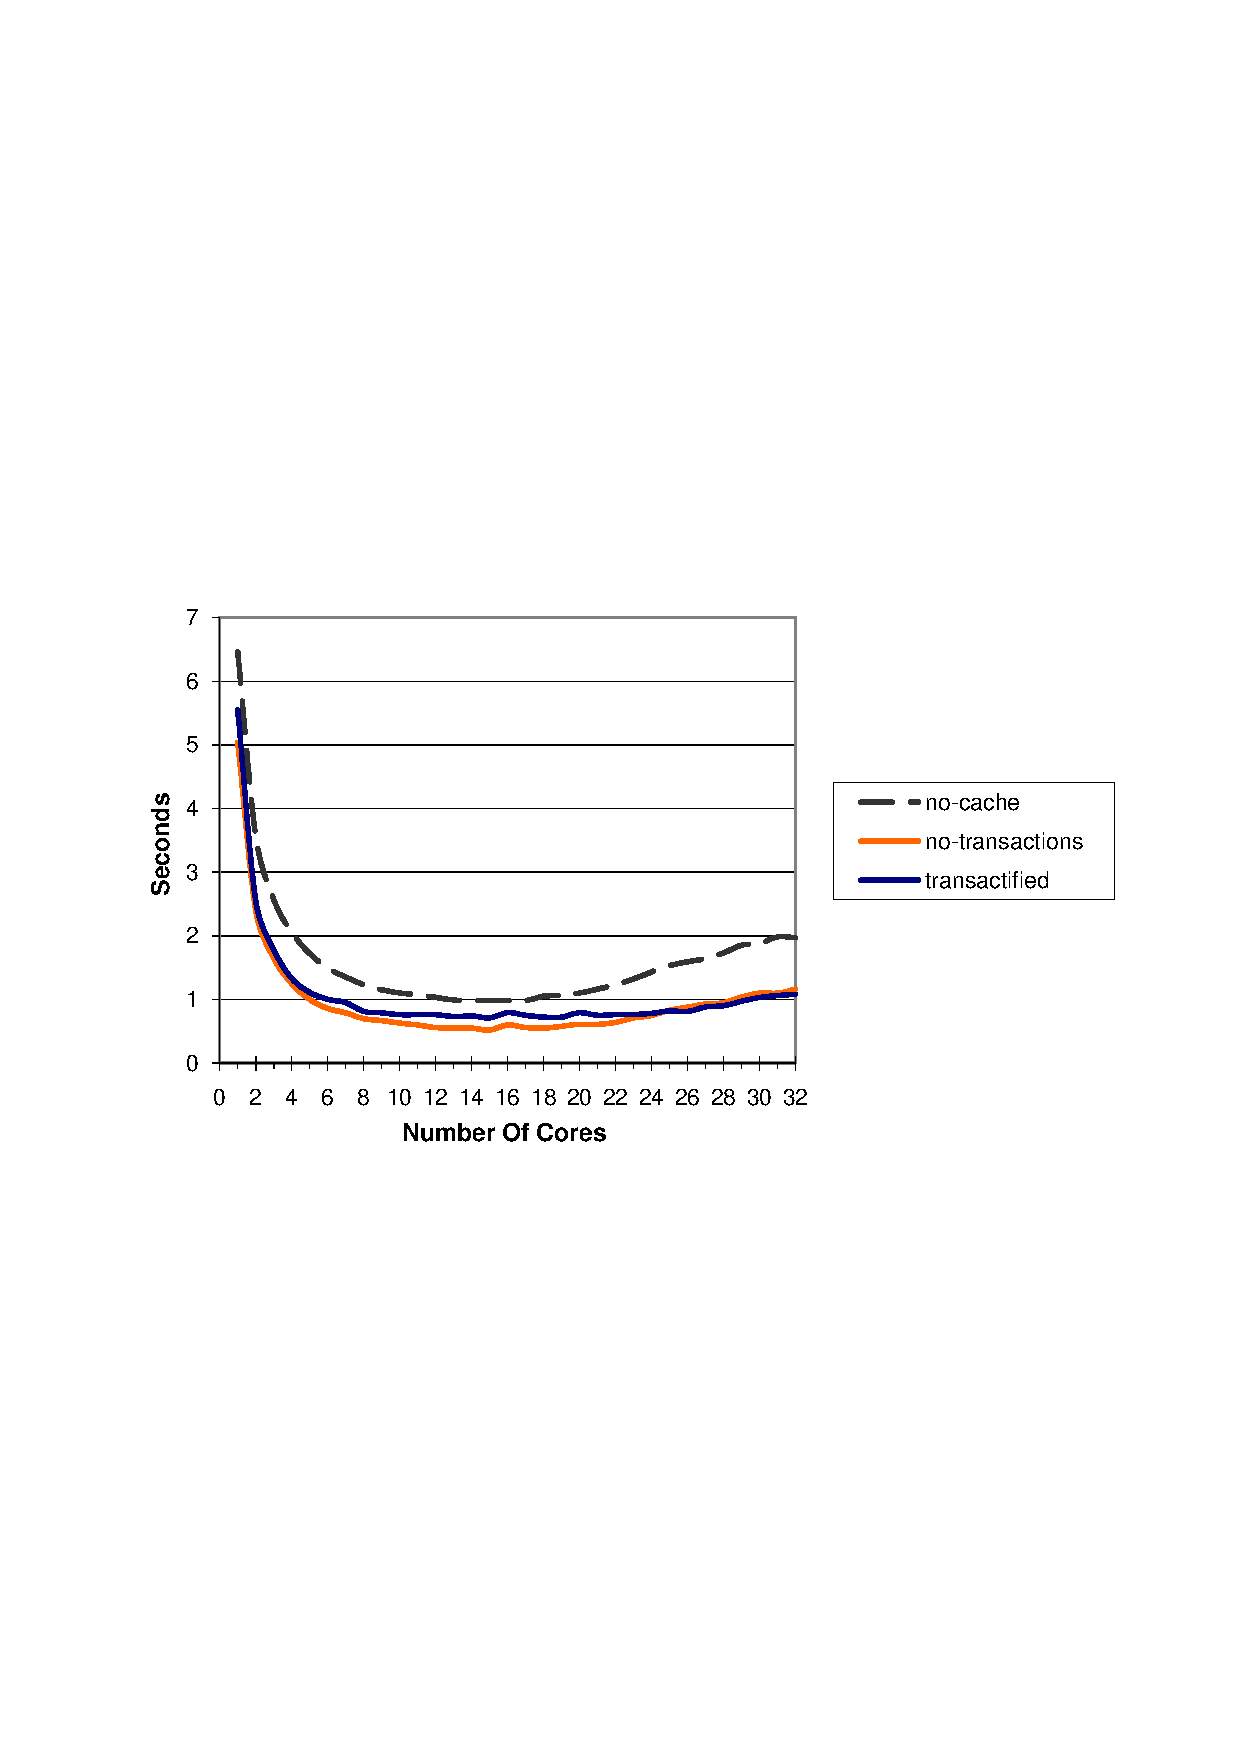
\includegraphics[width=8.5cm, trim=1cm 9.5cm 0 10.6cm]{response-time-client-server-1.pdf}
  \label{fig:response-time-1}
 }
 \caption{Medium locality workload ($s = 1$). 
 STM incurs a performance penalty, but the cache provides an improvement.}
\end{figure*}

With more representative locality, such as $s=1$,
(Figures~\ref{fig:request-throughput-1} and ~\ref{fig:response-time-1}), caching
is beneficial. The overhead of STM is still significant, but its performance is
better than when not using a cache at all. 

\begin{figure*}
 \centering
 \subfigure[Request throughput]{
  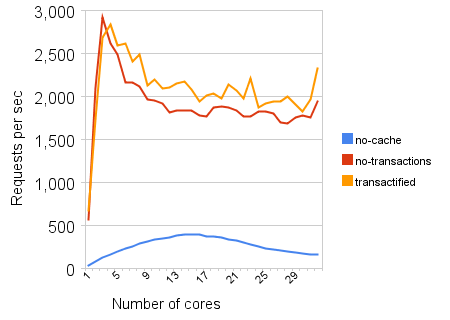
\includegraphics[width=8.5cm, trim=1cm 9.5cm 0 10.6cm]{transaction-rate-client-server-2.pdf}
  \label{fig:request-throughput-2}
 }
 \hfill
 \subfigure[Average response time]{
  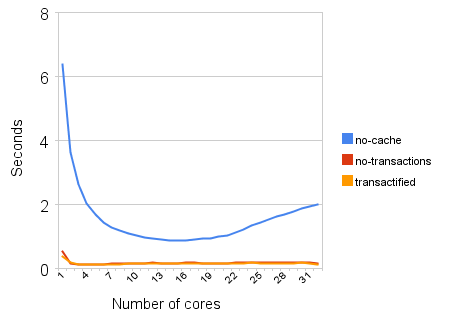
\includegraphics[width=8.5cm, trim=1cm 9.5cm 0 10.6cm]{response-time-client-server-2.pdf}
  \label{fig:response-time-2}
 }
 \caption{High locality workload ($s = 2$). The cache is vital, and 
 the STM version works best.}
\end{figure*}

With even higher locality ($s=2$), the contention on the cache is high even with
small number of cores. The results of the high locality experiments are shown
in Figures~\ref{fig:request-throughput-2} and~\ref{fig:response-time-2}.
In this case, caching provides major performance
benefits, increasing throughput by a factor of four. Here, the two 
cache-based versions exhibit close results, with a small yet consistent
advantage to the STM version.

In all the experiments described above, performance begins to decrease
beyond a certain number of cores. This number becomes smaller as 
the locality increases, albeit it occurs at a higher throughput when
there is more locality. This occurs due to the increased competition
among the cores over the shared resources. In particular, in the 
transactified version, the abort rate rises with the number of cores,
as we show below. 

We further note that in all workloads, there is a number of cores for which the
transactified version performs better than the original version. This might be
due to the advantage STM has over course-grained locking -- the fact that
transactions only collide when they access the same memory, while the
non-transactified version requires the same lock for all requests.

\begin{figure*}
 \centering
 \subfigure[Request throughput]{
  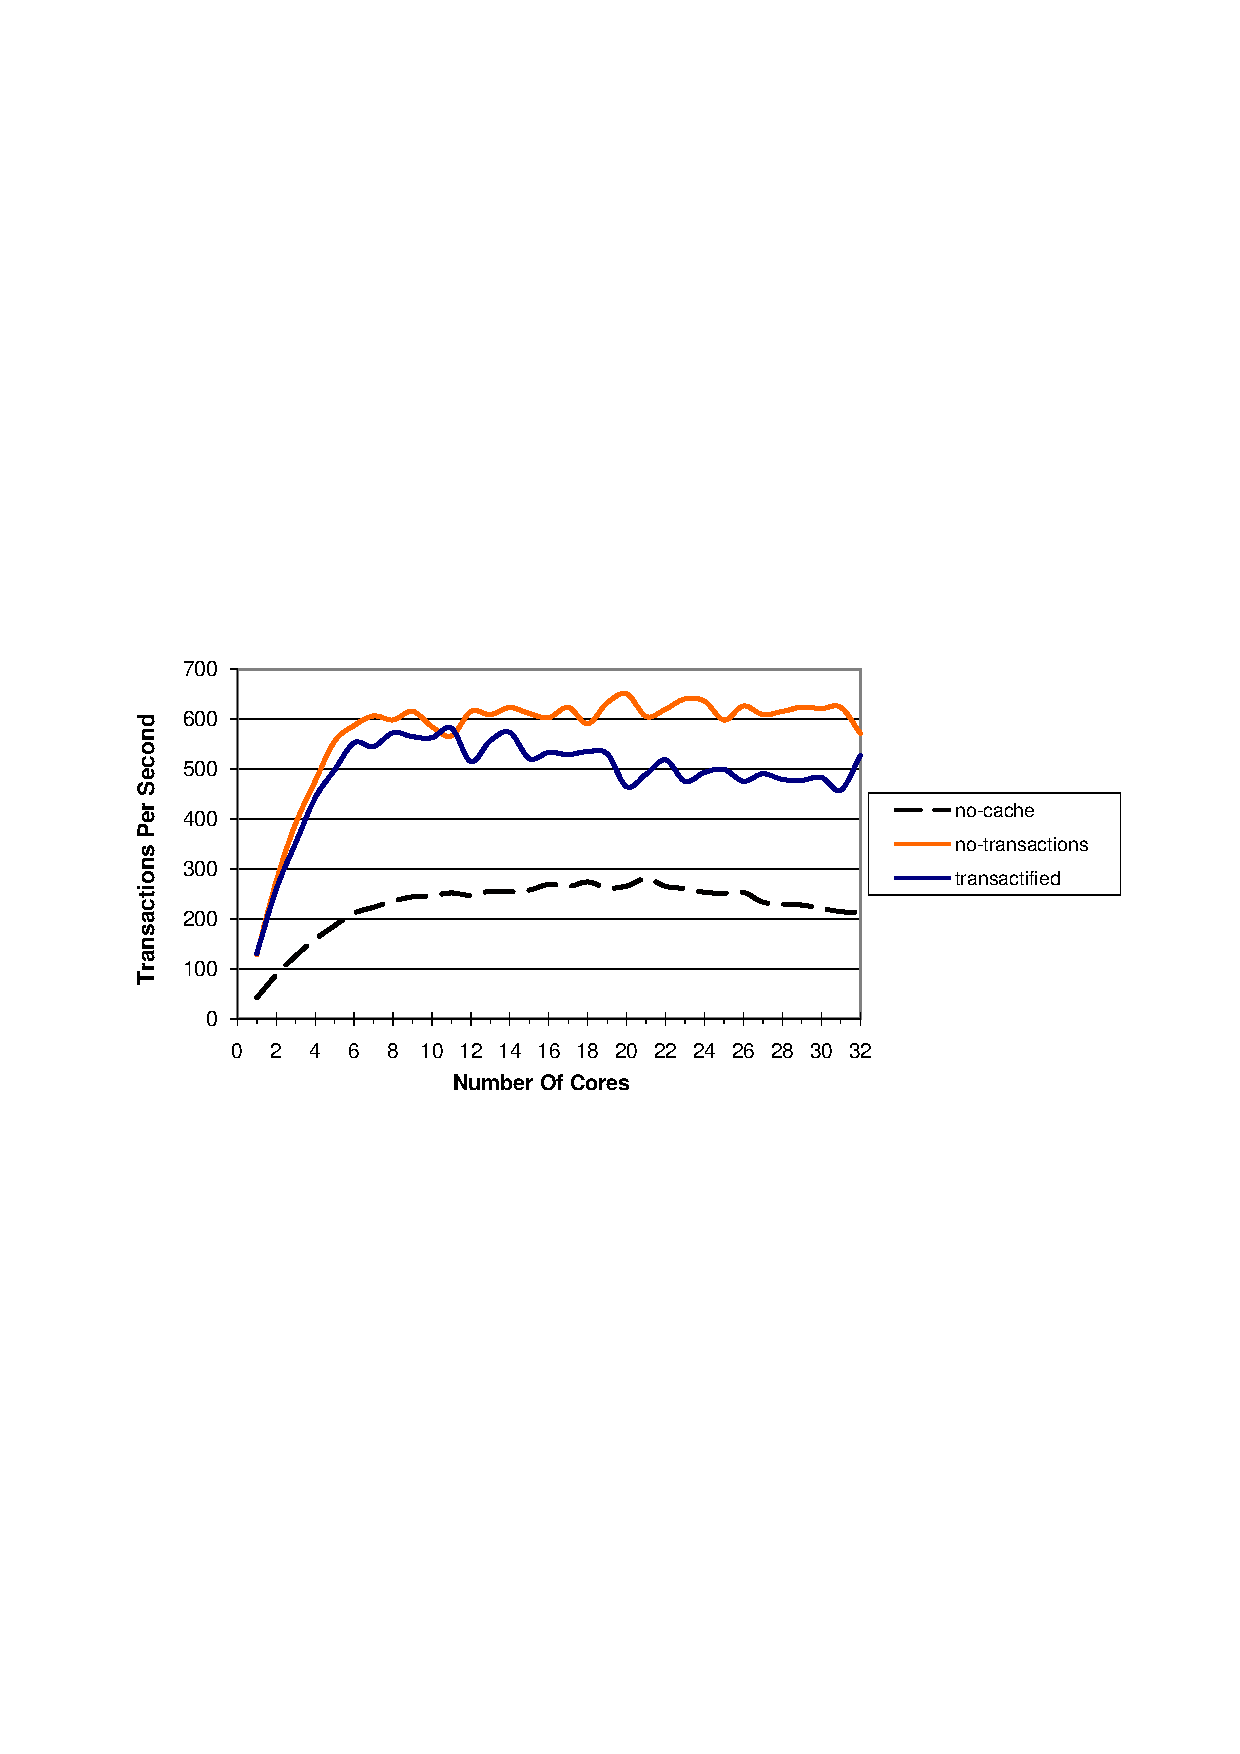
\includegraphics[width=8.5cm, trim=1cm 9.5cm 0 10.6cm]{transaction-rate-single-process.pdf}
  \label{fig:one-process-request-throughput}
 }
 \hfill
 \subfigure[Abort rate]{
  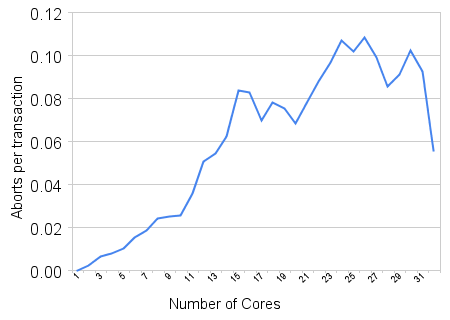
\includegraphics[width=8.5cm, trim=1cm 9.5cm 0 10.6cm]{abort-rate.pdf}
  \label{fig:one-process-abort-rate}
 }
 \caption{Medium locality workload ($s = 1$), Apache in single-process mode.
 The abort rate increases with the number of cores, which explains the decline 
 in the transaction rate.}
\end{figure*}

In order to investigate this decrease in throughput, we wanted to show the
transaction abort rate for these experiments. Unfortunately, as noted in
Section~\ref{sec:wishlist-statistics}, Intel STM's statistics mechanism
is unable to work with multiple processes. We therefore ran an additional
experiment, with Apache in a single process debugging mode, in order to collect
internal data about the transactions. 

We ran this single-process experiment with the medium locality workload,
that is, with $s=1$. Surprisingly, we see
in Figure~\ref{fig:one-process-request-throughput} that the
throughput of both the original and the STM version improve in this mode.
This suggests that Apache's multi-process mode is somehow not supported
well on our machines. Nevertheless, as before, neither version is able to 
benefit from the maximum allowed parallelism of the machine. 

Figure~\ref{fig:one-process-abort-rate} shows the average number of aborts
per transaction for the experiment with the transactified version. 
The increase in the abort rate explains the decrease in the request
throughput. At first, the abort rate increases gradually, 
and the benefit of having more cores available outweighs it.
But after about eight cores, the increase in the abort rate dominates,
so that there is little benefit in using more cores. 

\section{Conclusions}\label{sec:conclusions}

We have reported on our experience in converting the Apache web 
server to use the TM paradigm instead of lock-based synchronization,
and the lessons we learned along the way. Our conclusions include:

\begin{itemize}

\item
In order to cope with the scale of the software, we had to restrict
our attention to a small part of it. 
Out of 340,000 lines of code in the Apache web server, the cache module
is comprised of only 6651 lines of code, of which we modified only 273. 
This highlights the importance of being able to modify only
encapsulated sections of the code, and inter-operating with legacy software,
which might still use locks.  Moreover, legacy systems often interact
with software libraries whose source code is unavailable. 

  \item Having commit handlers in the STM system is not only needed for creating
efficient open transactions, but can also aid the process of transactifying
legacy code.

  \item It is important to work on real-world applications, as they
may reveal challenges resulting from engineering problems and not only
algorithmic and theoretical problems.

\end{itemize}

We next indicate two future directions that may follow on our work. 
First, there are many STM systems currently available, and one immediate direction
would be to compare them using this new TM benchmark. Doing so would require writing
plugins for existing TM system to match Intel's TM ABI. 
A second direction is to transactify additional 
legacy applications, following the methods we used.

%\appendix
%\section{Appendix Title}

% This is the text of the appendix, if you need one.

\acks

The authors would like to thank Torvald Riegel from the Transactional Memory Research
group at Dresden University of Technology, for is help with {\sc Tanger}. 
This work was partially supported by Semiconductors Research
Corporation (SRC), Intel, and the Israeli Ministry of Science
Knowledge Center on Chip Multiprocessors.

\bibliographystyle{plainnat}

%\begin{thebibliography}{}
%
%\bibitem{smith02}
%Smith, P. Q. reference text
%
%\end{thebibliography}

\bibliography{references}

\end{document}

